\newcommand{\prototype}[1]{
	\begin{tabularx}{\textwidth}{|l|X|}
	\hline
	Prototype&\texttt{#1} \\
	\hline
	\end{tabularx}
}

\chapter{Linux I/O Layer}

\section{Introduction}

This chapter will describe the Linux I/O layer. In order to develop a filesystem, you should understand how a Linux system interacts with files, devices and filesystems. This chapter will shed light on Linux I/O internals.

It is surprising to see how close Linux tries to follow the original UNIX architecture, as outlined in \cite{TDotUOS}. This book is a good reference to understand the algorithms and major design ideas (for example, of the cache code), but not the actual implementation.

Only the actual filesystem layer itself will be described in detail, because it is the most important for this project. For a complete overview of the I/O path, refer to Job Wildschut's technical graduation report: Linux IO Performance, which sheds light on the internals. \cite{LIOP}

\newpage

\section{Overview}

Linux I/O can be summarized in the following image:

\begin{figure}[h]
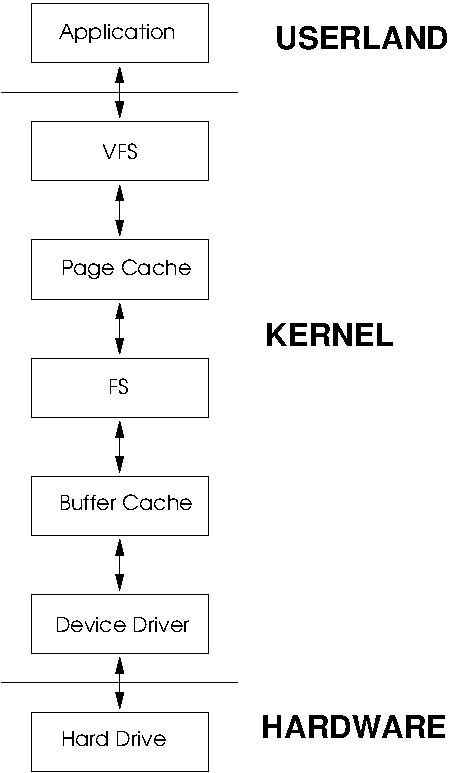
\includegraphics[height=10cm]{io-overview}
\caption{Summary of Linux I/O layers}
\end{figure}

Whenever a file is accessed, the request is passed down to the Virtual Filesystem. The VFS is actually a generic, filesystem independent interface which translates system calls, like open(2), read(2) etc to specific filesystem functions.

The page cache provides an uniform interface to file reading/writing, which handles functions like mmap(2). It provides all functionality in generic functions, relying only on the filesystem to provide buffers (using the buffer cache) for the actual data on disk. All other functionality is implemented by the filesystem code itself, described below.

The filesystem will receive VFS and page-cache requests and resolve them to I/O requests. These I/O requests are handled by the buffer cache, which will read blocks from a device and place them in a cache buffer. Modified buffers are written back to the disk as needed. The filesystem must conform to an interface as defined in the VFS layer. This layer is described in the VFS layer section later on.

The device driver is the device-dependent layer, which will handle the Linux I/O request and translate it into a device request.

\section{VFS layer}

This section will describe the VFS layer as well as the connection between the VFS and the page cache.

Before a filesystem is known by the kernel, it must be registered. This must be done using the \texttt{register\_filesystem()} call, which takes a \texttt{struct file\_system\_type} argument.

The most important member of this struct is \texttt{get\_sb} (get superblock), which points to a function which Linux will call whenever it tries to mount a filesystem of this type. This function must setup the \texttt{struct super\_block} which is passed along with it.

\subsection{Superblock operations}

\begin{verbatim}
static struct super_operations lime_sops = {
 .alloc_inode   = lime_alloc_inode,
 .destroy_inode = lime_destroy_inode,
 .read_inode    = lime_read_inode,
 .write_inode   = lime_write_inode,
 .put_super     = lime_put_super,
 .write_super   = lime_write_super,
 .statfs        = lime_statfs,
};
\end{verbatim}

The superblock operations structure contains the more low-level functions for a filesystem. These are basic operations such as inode management.

Dealing with files/directories will be done using the directory operations of the root inode (\texttt{sb-$>$s\_root} must always be set to the root inode), which will be covered in section \ref{dirops}.

\subsubsection{alloc\_inode}

\prototype{struct inode* alloc\_inode (struct super\_block* sb)}

Used to allocate an inode. The function should call the generic function \texttt{new\_inode} to allocate an inode and initialize it with filesystem-specific data.

\subsubsection{destroy\_inode}

\prototype{void destroy\_inode (struct inode* inode)}

The opposite of \texttt{alloc\_node}, this function must clean up the extra inode information. The inode itself must \emph{not} be destroyed, the VFS will take care of this.

\subsubsection{read\_inode}

\prototype{void read\_inode (struct inode* inode)}

Called whenever an inode structure must be filled, the inode to read is specified in \texttt{inode-$>$i\_ino}. Of all inode structure members, a few deserve special attention:

\texttt{inode-$>$i\_fop} is a pointer to an operations structure, which contains pointers to functions used for actual file/directory manipulation. These file operations are outlined in section \ref{fileops}, the directory operations can be found in \ref{dirops}.

\texttt{inode-$>$i\_op} is a pointer to an inode operations structure, which contains pointers to functions only needed for directory operations. These functions can be found in section \ref{inodeops}.

Should this operation fail, \texttt{make\_bad\_inode(inode)} must be used in order to invalidate the inode.

\subsubsection{write\_inode}

\prototype{void write\_inode (struct inode* inode, int synchronous)}

This will write inode data to the disk. The parameter indicates whether the data must be written synchronous, but is not implemented by most filesystems.

\subsubsection{put\_super}

\prototype{void put\_super (struct super\_block* sb)}

This will be called when the VFS unmounts the filesystem. Normally, a filesystem should update the on-disk superblock when the filesystem is dirty.

\subsubsection{write\_super}

\prototype{void write\_super (struct super\_block* sb)}

Called whenever the superblock needs to be written to the disk. This is for instance used while performing a sync(1) or fsync(2).

\subsubsection{statfs}

\prototype{int statfs (struct super\_block* sb, struct kstatfs* buf)}

Used to query used/free space/inode information. \texttt{struct kstatfs} can be found in \texttt{include/linux/statfs.h}, which must be filled by this function.

\subsection{Directory operations}
\label{dirops}

\begin{verbatim}
struct file_operations lime_dir_ops = {
 .read    = generic_read_dir,
 .readdir = lime_readdir,
 .fsync   = file_fsync,
};
\end{verbatim}

The functions outlined here are only used for directory inodes. Only \texttt{readdir} needs to be implemented (for it is very filesystem specific), the other functions call generic VFS functions which are suitable for most filesystems.

\subsubsection{readdir}

\prototype{int readdir (struct file* filp, void* dirent, filldir\_t filldir)}

Called to retrieve files in a directory (directory inode is \\
\texttt{filp-$>$f\_dentry-$>$d\_inode}), starting from offset \texttt{filp-$>$f\_pos}. This offset must be updated after new entries are passed, so the VFS knows which offset it must query to obtain the next directory entry.

\texttt{filldir} is the function to be called for each result, a prototype can be found in \texttt{include/linux/fs.h}.

\subsection{Inode operations}
\label{inodeops}

\begin{verbatim}
struct inode_operations lime_dir_inode_ops = {
 .create    = lime_create,
 .lookup    = lime_lookup,
 .link      = lime_link,
 .unlink    = lime_unlink,
 .symlink   = lime_symlink,
 .mkdir     = lime_mkdir,
 .rmdir     = lime_rmdir,
 .rename    = lime_rename,
};
\end{verbatim}
 
Misleading as the name may be, inode operations are mainly used in a directory context. They are mainly invoked for creating new inodes and looking up inode information. File inodes use so-called file operations which are outlined in section \ref{fileops}.

\subsubsection{create}

\prototype{int create (struct inode* dir, struct dentry* dentry, int mode, struct nameidata* nd)}

Creates a new file in \texttt{dir}, with name \texttt{dentry-$>$d\_name.name} and mode \texttt{mode}. On success, this function must call \texttt{d\_instantiate()} to add the created dentry to the cache.

\subsubsection{lookup}

\prototype{struct dentry* lookup (struct inode* dir, struct dentry* dentry, struct nameidata* nd)}

Called to retrieve the inode number from a filename (\texttt{dentry-$>$d\_name.name}) in a directory (directory inode is in \texttt{dir-$>$d\_ino}). On success, the inode found should be read (using \texttt{iget}) and added to the inode cache (using \texttt{d\_add}).

\subsubsection{link}

\prototype{int link (struct dentry* old\_dentry, struct inode* dir, struct dentry* dentry)}

Create a hard link from \texttt{old\_dentry} to \texttt{dentry} in directory \texttt{dir}. Inode information from \texttt{old\_dentry} can be copied over to the new inode as needed.

\subsubsection{unlink}

\prototype{int unlink (struct inode* dir, struct dentry* dentry)}

Removes an inode by name (\texttt{dentry-$>$d\_name.name}) in directory \texttt{dir}.

\subsubsection{symlink}

\prototype{int symlink (struct inode* dir, struct dentry* dentry, const char* symname)}

Create a soft link by name (\texttt{dentry-$>$d\_name.name}) in directory \texttt{dir}. The soft link should point to \texttt{symname}.

\subsubsection{mkdir}

\prototype{int mkdir (struct inode* dir, struct dentry* dentry, int mode)}

Create a new directory in parent directory \texttt{dir}. The directory name is passed in \texttt{dentry-$>$d\_name.name} and the mode in \texttt{mode}.

\subsubsection{rmdir}

\prototype{int rmdir (struct inode* dir, struct dentry* dentry)}

Removes directory named \texttt{dentry-$>$d\_name.name} from parent directory \texttt{dir}. This function must check whether the supplied directory is empty, and return \texttt{-ENOTEMPTY} if not.

\subsubsection{rename}

\prototype{int rename (struct inode* old\_dir, struct dentry* old\_dentry, struct inode* new\_dir, struct dentry* new\_dentry)}

This will rename entry \texttt{old\_dentry-$>$d\_name.name} in directory \texttt{old\_dir} to entry \texttt{new\_dentry-$>$d\_name.name} in directory \texttt{new\_dir}. This function must ensure \texttt{new\_dentry-$>$d\_name} doesn't already exist before continuing.

\subsection{File operations}
\label{fileops}

\begin{verbatim}
struct file_operations lime_file_ops = {
 .llseek     = generic_file_llseek,
 .read       = generic_file_read,
 .write      = generic_file_write,
 .mmap       = generic_file_mmap,
 .fsync      = file_fsync,
 .sendfile   = generic_file_sendfile
};
\end{verbatim}

These functions usually refer to generic VFS functions. All disk-based filesystems use the page cache for data reading/writing. The \texttt{generic\_file\_read} and \texttt{generic\_file\_write} functions use the inode's \texttt{i\_mapping-$>$a\_ops} to refer to the address space operations. These are documented below:

\begin{verbatim}
struct address_space_operations lime_aops = {
 .readpage      = lime_readpage,
 .writepage     = lime_writepage,
 .prepare_write = lime_prepare_write,
 .commit_write  = generic_commit_write
};
\end{verbatim}

The functions listed here use generic VFS calls, which ultimately only need a single function from the filesystem: the \texttt{get\_block} function, which is fully explained in \cite{TDotUOS}. A more Linux-specific explanation is given in the next paragraph.

\subsubsection{get\_block}

\label{getblk}
\prototype{int get\_block (struct inode* inode, sector\_t iblock, struct buffer\_head* bh\_result, int create)}

This function is passed to generic calls (these are \texttt{block\_read\_full\_page()} and \texttt{block\_write\_full\_page()}), which expects it to return a mapped buffer to a requested block within a file (the size of a block must be set on initialization time, using \texttt{sb\_set\_blocksize}).

The filesystem should allocate a new block if the the \texttt{create} flag is non-zero.

\section{ABISS}

\wi{ABISS}, or the Active Block I/O Scheduling System (as outlined in \cite{ABISS}) is a system designed to provide guaranteed read- and write performance to applications. The application issues a request to ABISS, in which a request is made for certain file bandwidth guarantees. ABISS will handle this by ordering writes and providing read-aheads as needed.

From a filesystem's point of view, some functions can be provided to ABISS, using the following structure:

\begin{verbatim}
struct abiss_fs_ops lime_fs_ops = {
 .get_block              = lime_do_get_block,
 .readpage               = lime_readpage,
 .alloc_unit             = lime_alloc_unit,
};
\end{verbatim}

The first function, \texttt{get\_block}, must be an entry point to the get block function as outlined in section \ref{getblk}. It is used to cache the logical block numbers, so no disk accesses are needed to look up blocks.

The second function, \texttt{readpage}, is the entry point to the file system's readpage function as outlined in section \ref{fileops}. This is used for the readahead functionality.

Finally, \texttt{alloc\_unit} must return the basic block allocation unit of the filesystem, in bytes.
